% Memory Is Signed -- single-source ICLR 2027 manuscript.
% Compile: pdflatex main.tex; pdflatex main.tex.
% Every measured number below is produced by plotting/extract_evidence.py from
% the repository JSON records; the verification report it prints is the
% provenance for Tables 1-6 and Figures 1-5. Unmeasured quantities are stated in
% prose as limitations and listed in DELIVERY_PACKAGE.md section 12; the
% manuscript contains no placeholders.
\documentclass{article}
\usepackage{iclr2027_conference,times}
\usepackage[T1]{fontenc}
\usepackage[utf8]{inputenc}
\usepackage{microtype}
\usepackage{amsmath,amssymb,mathtools}
\usepackage{booktabs,array,multirow}
\usepackage{graphicx,xcolor}
\usepackage{tikz}
\usetikzlibrary{arrows.meta,positioning,fit,calc,backgrounds}
% float.sty supplies the algorithm float; the body is typeset directly so the
% listing stays editable and needs no algorithm bundle in the TeX Live install.
\usepackage{float}
\newfloat{algorithm}{t}{loa}
\floatname{algorithm}{Algorithm}
\usepackage{url}
\usepackage[hidelinks]{hyperref}
\hypersetup{pdftitle={Memory Is Signed: Causal Credit Measurement in Vision-Language GUI Agents},pdfauthor={Anonymous authors}}
\newcommand{\method}{\textsc{Sigma}}
\newcommand{\E}{\mathbb{E}}
\newcommand{\R}{\mathbb{R}}
\newcommand{\sg}{\operatorname{sg}}
\newcommand{\KL}{\operatorname{KL}}
\newcolumntype{L}[1]{>{\raggedright\arraybackslash}p{#1}}
\DeclareMathOperator*{\argmax}{arg\,max}
\DeclareMathOperator*{\argmin}{arg\,min}
\definecolor{ink}{HTML}{183246}
\definecolor{ink2}{HTML}{465A66}
\definecolor{useful}{HTML}{2A78D6}
\definecolor{harmful}{HTML}{E34948}
\definecolor{neutral}{HTML}{898781}
\definecolor{muted}{HTML}{898781}
\definecolor{pale}{HTML}{F4F6F7}
\definecolor{linegray}{HTML}{C3CDD2}
% No geometry, font-size, line-spacing or style-file overrides.
\title{Memory Is Signed: Causal Credit Measurement\\for Historical Representations\\in Vision-Language GUI Agents}
\author{Anonymous authors}
%\iclrfinalcopy
\begin{document}
\maketitle

\begin{abstract}
A GUI agent that keeps its history can still act on a record it has already
superseded, with the correcting evidence sitting in the same context window.
We show that this failure is a property of the model's \emph{historical
key--value representations}, and that its direction is measurable and
predictable. Replacing one historical key span in a frozen vision--language
model, while holding screenshots, action candidates and recipient positions
fixed, moves critical-decision accuracy from 60\% to 100\% when the replaced
span is a superseded update, and from 60\% to 0\% when it is the latest one.
Across 200 controlled histories and 1{,}000 matched replacements, superseded
updates carry negative credit in 92\% of cases and latest updates carry positive
credit in 98.5\%, while matched reference spans are indistinguishable from zero;
181 of 200 prefixes exhibit both signs at once. The sign is set by a block's
relation to the current decision, not by its age: an initial record is just as
old as the superseded update it precedes, yet its credit is weakly positive. We
then show that this quantity is invisible to ordinary training signals. On 400
paired MiniWoB cases, return-weighted training raises the candidate margin the
objective optimises from $0.1502$ to $0.1711$ while completing no more tasks
than the frozen base and four fewer than plain action cross-entropy. We
introduce \method, a framework that treats measured replacement effects as
supervision: a history-aware controller predicts signed credit from clean prefix
features and conditions a low-rank correction on historical key--value spans.
\method\ operationalises the measurement; its end-task benefit is not yet
established, and we report that boundary explicitly.
\end{abstract}

\section{Introduction}
\label{sec:intro}

An agent reads an order, observes a correction, and later submits the order
using the old value. Nothing was lost. Both the original record and the
correction are in the context window, and the newest screenshot is the one in
front of the model. What failed was not retention but \emph{influence}: a
historical representation that should have stopped affecting the decision did
not.

GUI agents are built to accumulate exactly this kind of state. Screenshots,
prior actions and past observations are concatenated into a growing prefix, and
the resulting key--value (KV) cache is carried forward as the agent's memory
\citep{wang2024awm,liu2026memgui}. The field's default assumption is that this
memory is monotone: more retained history is more capability, and the way to
improve an agent's use of its past is to improve what it does with the
\emph{current} screen. Memory research in this setting has accordingly focused
on what to retrieve and how much to trust it \citep{wang2024awm,zhang2026focusmem}.
The complementary question---whether a representation that is still present
should still be allowed to vote---is rarely asked, because it has no obvious
observable. Task success is a single scalar at the end of an episode and
attributes nothing to any particular part of the past.

This paper measures that contribution directly. Our starting point is a
controlled setting in which the failure is unambiguous, and which we can
perturb one representation at a time.

\paragraph{The problematic observation.}
\emph{Interference Chain} presents a frozen vision--language model (VLM) with a
sequence of GUI updates: an initial record, a reference observation, an update
that a later observation supersedes, a second reference, and a latest update.
The final screen offers eight neutrally named action slots, and selecting the
correct slot requires relating the historical record to the current screen.
Screenshots, action candidates, token counts and target positions are held
fixed throughout. The only thing we change is which historical key span the
decoder attends over: we replace a selected span with a matched one from
elsewhere in the same prefix, before rotary position encoding, so the
replacement inherits the recipient's positions.

The result is in Figure~\ref{fig:intervention}. The unmodified model selects the
correct action in 6 of 10 paired prefixes. Replacing the \emph{superseded}
update repairs all four failures, reaching 10 of 10. Replacing the
\emph{latest} update destroys all six successes, reaching 0 of 10. Replacing
either matched reference leaves accuracy at 6 of 10, and replacing the initial
record---an equally old span---moves it only to 5 of 10. Identical pixels, opposite
outcomes.

% Figure 1 float: the hero intervention. Plotting code lives in
% plotting/fig1_intervention.py; this file only wraps it for the manuscript.
\begin{figure}[tbp]
\centering
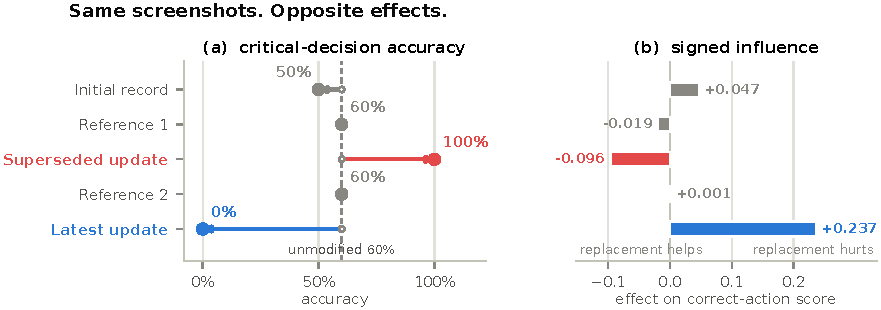
\includegraphics[width=\linewidth]{figures/fig1_intervention.pdf}
\caption{\textbf{One historical key span decides the action.} Ten paired
prefixes, frozen Qwen2.5-VL-3B-Instruct, decoder key-projection outputs at
layers 12--23. Screenshots, candidate slots, token counts and recipient
positions are identical across rows; only the source of one historical block's
key span changes. (a) Critical-decision accuracy after replacing that block with
a matched donor. (b) The same replacement's signed effect on the correct-action
score of Eq.~\eqref{eq:act}, in the units of Table~\ref{tab:pilot}. Replacing
the superseded update repairs every failure; replacing the latest update
destroys every success; the two matched references leave behaviour unchanged and
the older initial record moves it by a single prefix. Age alone therefore does
not produce the pattern.}
\label{fig:intervention}
\end{figure}


\paragraph{What this rules out.}
The two updates differ in age by one observation, and the initial record is
older than both, so recency cannot generate the pattern. Both updates are
semantically similar records about the same task, so content alone cannot
either. What separates them is their relation to the current decision: one has
been superseded and one has not. Age and content are the two signals a memory
system can observe without intervening on the model, and neither predicts the
sign we measure.

\paragraph{The measurement does not reduce to confidence.}
If interference were merely weak or noisy memory use, better-optimised action
scores would fix it. They do not. On 400 paired MiniWoB cases
(Figure~\ref{fig:divergence}), return-weighted training raises the mean top-1
candidate margin---the quantity such objectives actually optimise---from
$0.1502$ to $0.1711$, the largest margin of any arm. It completes 330 of 400
tasks: one more than the frozen base, and three fewer than plain action
cross-entropy, which has the \emph{lowest} margin of all arms at $0.1471$. The
same decoupling appears in our own precursor runs, where return-conditioned KV
adaptation lifted a held-out return margin from $0.1965$ to $0.2598$ while
leaving top-1 action ranking at $0.50$ for every arm including the frozen base.
An objective can sharpen its own score without changing what the agent does.
Reading memory quality off that score is therefore not merely imprecise; it can
point the wrong way.

\paragraph{Contributions.}
(i) We introduce a matched-replacement measurement of \emph{signed causal
memory credit} for historical KV spans in a frozen GUI VLM, and show the sign
is stable and large where the phenomenon predicts and null where it does not
(\S\ref{sec:credit}). (ii) We show the effect is per-instance, not an artifact
of averaging: 181 of 200 prefixes show the superseded and latest signs
simultaneously, and each update block is separable from the reference blocks
with AUROC $0.86$ and $0.94$ (\S\ref{sec:credit}). (iii) We show that this
signal is not recoverable from the training objectives currently used for GUI
memory, using a failure of our own precursor method as evidence
(\S\ref{sec:divergence}). (iv) We give \method, which turns measured credit into
supervision for a history-aware controller and a gated low-rank correction
(\S\ref{sec:method}).

\section{Measuring the Contribution of a Memory}
\label{sec:method}

\subsection{Decision prefixes and matched memory credit}

At GUI step $t$, the agent observes $h_t=(x,o_{1:t},a_{1:t-1})$, where $x$ is
the user instruction and $o_i$ a screenshot. The frozen VLM induces a memory
$M_t=F_\theta(h_t)$. For selected decoder layers $\mathcal L$, each historical
visual block is indexed by
\begin{equation}
 m_{t,j}=\{K_{\ell,j},V_{\ell,j}\}_{\ell\in\mathcal L},
 \qquad K_{\ell,j},V_{\ell,j}\in\R^{n_j\times d_\ell}.
 \label{eq:memory}
\end{equation}
Heads are flattened into $d_\ell$ for notation. Current-screen tokens and
generated action tokens lie outside the historical intervention mask.

Let $\mathcal P_{j,d}$ replace block $j$ with a shape-compatible donor $d$ drawn
from the same prefix. For a fixed decision utility $u$, the credit of block $j$
is
\begin{equation}
 c^u_{t,j}=u(h_t;M_t)-\E_{d\sim\mathcal D_{t,j}}
       \big[u(h_t;\mathcal P_{j,d}(M_t))\big].
 \label{eq:credit}
\end{equation}
Positive credit means the original block serves the utility better than its
matched replacements; negative credit means the replacements are preferable. The
donor distribution, layer set and utility are part of the estimand, and the
quantity is conditional: the same screenshot can carry a different sign after
another observation or under a different goal. It is not an intrinsic label.

\subsection{Three utilities, three claims}

The intervention operator is shared but its target depends on available
supervision, and we keep three utilities separate throughout.

\paragraph{Action-score effect.} For a validated target action $a^\star$ of
length $L$, the diagnostic score is the mean teacher-forced token
log-probability
\begin{equation}
 u_{\mathrm{act}}(h;M)=\frac{1}{L}\sum_{k=1}^{L}
 \log\pi_\theta(a_k^\star\mid h,M,a_{<k}^\star).
 \label{eq:act}
\end{equation}
Length normalisation makes this a ranking score, not the log-probability of an
executable trajectory. This is the utility used in the ten-prefix pilot.

\paragraph{Candidate-value effect.} Given a fixed candidate set $\mathcal C(h)$,
scores $s_a$ from Eq.~\eqref{eq:act}, and independently assigned continuation
values $\bar Q(h,a)$,
\begin{equation}
 p^\mathcal C_M(a\mid h)=\frac{\exp(s_a/T_c)}{\sum_{b\in\mathcal C(h)}\exp(s_b/T_c)},
 \qquad
 u_{\mathrm{val}}(h;M)=\sum_{a\in\mathcal C(h)}p^\mathcal C_M(a\mid h)\bar Q(h,a).
 \label{eq:val}
\end{equation}
The 200-prefix study uses this proxy. Its values describe a redistribution of
probability among the specified candidates and depend on candidate coverage and
on the continuation policy behind $\bar Q$. They are \emph{not} on the same
scale as Eq.~\eqref{eq:act}, and we never compare the two numerically.

\paragraph{Trajectory-return effect.} For a restorable environment state $s_t$,
\begin{equation}
 u_{\mathrm{roll}}(h_t,s_t;M_t)
   =\E_{\tau_{t:T}\sim P_\theta(\cdot\mid h_t,s_t;\operatorname{do}(M_t))}
        [R(\tau_{t:T})].
 \label{eq:roll}
\end{equation}
This is the performance-linked extension. Neither Eq.~\eqref{eq:act} nor
Eq.~\eqref{eq:val} substitutes for it when reporting online success, and the
estimator's design is given in Appendix~\ref{app:protocol}.

\subsection{Measuring credit without target leakage}
\label{sec:teacher}

Teacher extraction starts from the observable prefix alone: it records visual
token spans, candidate-independent decision features, and donor tensors. Each
target is patched in a separate evaluation, effects are averaged over admissible
donors, and a donor is never the target itself. Recipient length and positions
are preserved; content and activation norms need not be. For the training
extractor, donors are frozen from a clean prefix pass so an earlier intervention
cannot alter a later donor. The within-forward diagnostic reported in
\S\ref{sec:interference} and this clean-donor variant are different protocols
and are recorded separately; we do not relabel the first as the second.

Training actions and evaluators may define labels but never controller inputs.
All candidates share prefix-only features, the recurrent state excludes
target-action tokens, and test-time control uses predicted credit without
correct actions or intervention-derived labels.

\section{Signed Credit Is Large, Stable, and Role-Determined}
\label{sec:credit}

\subsection{The ten-prefix intervention}
\label{sec:interference}

Table~\ref{tab:pilot} and Figure~\ref{fig:intervention} report the pilot in
full. We use Qwen2.5-VL-3B-Instruct \citep{bai2025qwen} with frozen parameters,
intervening on historical visual tokens at the decoder's key-projection outputs
in layers 12--23 (zero-based, of 36). This follows the activation-patching
principle of comparing controlled internal substitutions
\citep{zhang2024patching}.

The diagnostic separates the roles cleanly on this sample: update-block sign
accuracy $1.0$, localisation of updates against references at AUROC $1.0$, and
reference neutrality accuracy $1.0$ at a tolerance of $0.025$. With ten paired
prefixes these are pilot-level statistics and we do not treat them as estimates
of a population. Their function is to establish that the protocol yields the
intended contrast at all, which licenses the larger study below.

\begin{table}[tbp]
\caption{\textbf{Ten-prefix matched replacement.} Accuracy is the
critical-decision accuracy over ten paired prefixes; the effect is the change in
the utility of Eq.~\eqref{eq:act} when that block is replaced. Sign convention:
a positive effect means the original block is preferable to its matched
replacement. References are patched with donors ``Reference~1'' and
``Reference~2'' respectively; update and initial blocks use a reference donor.
The two reference rows are the control for the intervention itself.}
\label{tab:pilot}
\centering
\small
\begin{tabular}{lrrr}
\toprule
Replaced block & Accuracy & Change & Signed effect $u_{\mathrm{act}}$\\
\midrule
\emph{unmodified model} & 0.60 & --- & ---\\
Initial record            & 0.50 & $-0.10$ & $+0.0469$\\
Reference 1               & 0.60 & $\phantom{-}0.00$ & $-0.0194$\\
\textbf{Superseded update}& \textbf{1.00} & $+0.40$ & $\mathbf{-0.0965}$\\
Reference 2               & 0.60 & $\phantom{-}0.00$ & $+0.0013$\\
\textbf{Latest update}    & \textbf{0.00} & $-0.60$ & $\mathbf{+0.2368}$\\
\bottomrule
\end{tabular}
\end{table}

\subsection{Two hundred histories}

The pilot leaves open whether the pattern survives scale. We extract credit for
all five blocks over 200 independently generated prefixes in a held-in template,
giving 1{,}000 matched-block measurements. Two reference donors are used for
non-reference blocks and one other reference donor for a reference block, so
reference neutrality is measured against a weaker control than the update blocks
are, and we treat it accordingly.

\begin{table}[tbp]
\caption{\textbf{Signed credit over 200 controlled histories.} The utility is
the candidate-value proxy of Eq.~\eqref{eq:val}, in candidate-value units;
these numbers are not comparable to the action-score effects of
Table~\ref{tab:pilot}. The interval is a bootstrap over prefixes ($B=4000$),
which is a cluster resample here because each prefix contributes exactly one
measurement per role. ``Positive'' is the fraction of the 200 per-prefix values
above zero.}
\label{tab:credit}
\centering
\small
\begin{tabular}{lrrrr}
\toprule
Historical block & Mean credit & Positive & Bootstrap 95\% & Mean $|$credit$|$\\
\midrule
Initial record       & $+0.000798$ & 55.0\% & $[+0.000178, +0.001429]$ & $0.003577$\\
Reference 1          & $+0.000103$ & 50.0\% & $[-0.000452, +0.000666]$ & $0.003035$\\
\textbf{Superseded update} & $\mathbf{-0.007612}$ & \textbf{8.0\%} & $[-0.008460, -0.006809]$ & $0.007834$\\
Reference 2          & $-0.000135$ & 50.0\% & $[-0.000762, +0.000464]$ & $0.003549$\\
\textbf{Latest update}     & $\mathbf{+0.011020}$ & \textbf{98.5\%} & $[+0.010167, +0.011894]$ & $0.011047$\\
\bottomrule
\end{tabular}
\end{table}

Table~\ref{tab:credit} and Figure~\ref{fig:credit} give the result. The two
update blocks carry large, opposite, precisely estimated credit: the superseded
update is negative in 92.0\% of prefixes and the latest update positive in
98.5\%, and both bootstrap intervals exclude zero by a wide margin. The three
non-update blocks do not. Reference means are within $1.4\times10^{-4}$ of zero
and their intervals straddle it.

The initial record is the informative case. It is older than the superseded
update, and a recency account predicts it should be at least as harmful. It is
not: its mean credit is weakly positive at $+0.000798$ with an interval
excluding zero, and it is positive in 55.0\% of prefixes. Whatever marks the
superseded update is therefore not its age.

\begin{figure}[tbp]
\centering
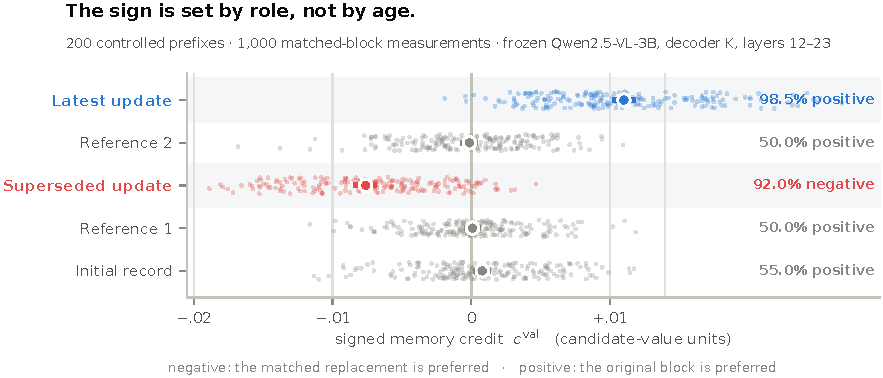
\includegraphics[width=\linewidth]{figures/fig2_signed_credit.pdf}
\caption{\textbf{Signed memory credit by block role over 200 controlled
prefixes.} Each faint point is one prefix's measurement for that block; the bold
marker is the mean and the bar a bootstrap 95\% interval over prefixes. Blue
denotes that the original block is preferable to its matched replacement, red
that the replacement is preferable. The two updates carry opposite signs at high
precision; the two matched references and the older initial record do not.
Values are in candidate-value units (Eq.~\eqref{eq:val}) and are not on the same
scale as Table~\ref{tab:pilot}.}
\label{fig:credit}
\end{figure}

\subsection{The effect is per-instance}

A near-zero mean can hide large effects of opposing sign, so the aggregate in
Table~\ref{tab:credit} is not by itself evidence that references are inert. We
therefore examine the joint pattern per prefix (Figure~\ref{fig:joint}).
Of the 200 prefixes, 181 (90.5\%) show the superseded update negative
\emph{and} the latest update positive simultaneously; the remaining 19 show one
of the two signs; none shows neither. The mean absolute effect sizes support the
same reading---references sit near $0.0030$--$0.0035$ while the updates sit at
$0.0078$ and $0.0110$---so reference neutrality is not an artifact of
cancellation.

Credit also localises each update block against the reference blocks
individually: AUROC $0.864$ for identifying the superseded update and $0.936$
for the latest, using the sign of a single block's credit with no access to
labels. A memory controller that had to decide which block to trust, using only
this measurement, would therefore be working from a signal with real
discriminative content rather than a role label copied from the data generator.

\begin{figure}[tbp]
\centering
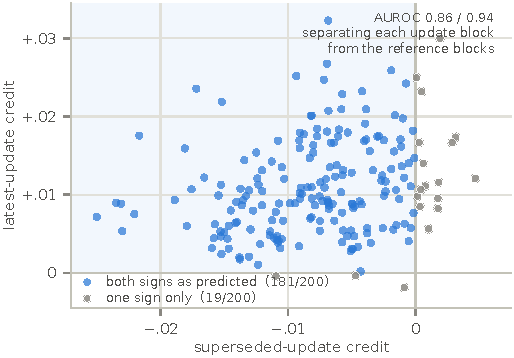
\includegraphics[width=0.62\linewidth]{figures/fig3_per_prefix.pdf}
\caption{\textbf{The opposing pattern holds per prefix.} Each point is one
controlled prefix, placed by its superseded-update credit (horizontal) and
latest-update credit (vertical). The shaded quadrant is the region a
role-driven account predicts. Blue points show both predicted signs, grey show
exactly one, and no prefix falls outside both. AUROC values are the
discriminability of each update block against the three non-update blocks from
credit sign alone.}
\label{fig:joint}
\end{figure}

\section{SIGMA: Turning Measurement into Adaptation}
\label{sec:sigma}

The measurement solves an identification problem: it says which historical
blocks deserve to influence the current decision. It does not say how to change
them. \method\ separates the two, using credit as supervision for a controller
and learning the correction direction from the action objective.

\subsection{History-aware credit distillation}
\label{sec:controller}

Memory utility depends on relationships among observations. A code in an old
record does not identify itself as superseded; a later update establishes that
relation. For each block we pool clean projection features over visual tokens
and selected layers, project them to a compact embedding $z_j$, and encode order:
\begin{equation}
 z_j=P_\phi(\operatorname{Pool}(m_{t,j})),\quad
 s_j=\operatorname{GRU}_\phi(z_j,s_{j-1}),\quad
 \hat c_{t,j}=f_\phi(z_j,s_J,q_t),
 \label{eq:controller}
\end{equation}
where $q_t$ is a clean prefix-only decision feature and the final recurrent
state lets an earlier block's prediction depend on all observations available at
step $t$. The GRU is a compact implementation choice, not a claim; it is
compared against an independent MLP and a small Transformer.

Targets are scaled by a positive constant $s_u$ fitted on training labels of the
same utility type, $\tilde c^u=c^u/s_u$; we never mix action-score and
candidate-value units or force the mean reference effect to zero. A neutrality
threshold $\epsilon_u$ defines a three-way target $y\in\{-,0,+\}$. With
nonnegative reliability weights $w_{t,j}$,
\begin{equation}
 \mathcal L_{\mathrm{credit}}=\E_{t,j}w_{t,j}
 \big[\operatorname{Huber}(\hat c_{t,j},\tilde c^u_{t,j})
       +\lambda_s\operatorname{CE}(p_\phi^{\mathrm{sign}},y_{t,j})\big]
       +\lambda_r\mathcal L_{\mathrm{rank}}.
 \label{eq:credit-loss}
\end{equation}
The ranking term compares clearly separated labels within a prefix; uncertain
donor comparisons are masked rather than converted into hard sign labels
(Appendix~\ref{app:loss}).

\subsection{From signed credit to a learned correction}
\label{sec:adapt}

A signed gate controls a low-rank residual on historical projection outputs. For
$X_{\ell,j}\in\{K_{\ell,j},V_{\ell,j}\}$ and learned $B_\ell\in\R^{d_\ell\times r}$,
$A_\ell\in\R^{r\times d_\ell}$,
\begin{equation}
 g_{t,j}=\tanh(\hat c_{t,j}/T_g),\qquad
 \Delta X_{\ell,j}=\frac{\alpha}{r}g_{t,j}X_{\ell,j}B_\ell A_\ell,
 \qquad X'_{\ell,j}=X_{\ell,j}+\Delta X_{\ell,j}.
 \label{eq:adapt}
\end{equation}
$B_\ell A_\ell$ is a general low-rank map, not an orthogonal projector, and a
negative gate does not universally reduce a block's attention contribution:
scaling a key can raise or lower its logit depending on the sign of
$q^\top k$. The sign of $c^u$ describes a \emph{finite replacement}, not the
derivative of utility along $XBA$; Appendix~\ref{app:loss} gives a two-point
counterexample. The credit loss therefore identifies what to adapt, while the
action objective learns how:
\begin{align}
 E_{\mathrm{KV}}&=\frac{1}{|\mathcal L|}\sum_{\ell\in\mathcal L}
   \frac{\sum_j\|\Delta X_{\ell,j}\|_F^2}{\sum_j n_jd_\ell},\label{eq:energy}\\
 \mathcal L_{\mathrm{SIGMA}}&=\mathcal L_{\mathrm{policy}}
       +\lambda_c\mathcal L_{\mathrm{credit}}+\lambda_E E_{\mathrm{KV}}.
 \label{eq:total}
\end{align}
$A_\ell$ is zero-initialised, so adaptation begins at the base policy. The
quadratic term regulates representation change; it is not an optimal-transport
objective over source and target distributions.

\subsection{Optimisation and deployment}

We first fit the controller to measured credit with the residual fixed at zero,
then optimise residual and controller jointly with Eq.~\eqref{eq:total},
retaining credit supervision so the gate does not become an unconstrained action
adapter. Backbone weights stay frozen. At interaction time a clean prefix pass
provides block and decision features, the controller predicts gates once, and a
second policy pass applies them before generating an action; new observations
produce a new prefix and new gates. This is state-dependent inference, not online
weight learning. Both passes are inside the runtime budget, and we do not claim
a latency reduction that no implementation has demonstrated.
Algorithm~\ref{alg:sigma} states the complete procedure.

% The SIGMA pipeline. Inline vector art so labels stay editable and no raster
% step enters the manuscript. Two lanes: (A) measures credit, (B) consumes it.
%
% Geometry note: the lane labels sit in a left gutter at x=-1.52 with anchor
% east, clear of the first box, whose left edge is at x=-1.30. An earlier
% revision placed them at x=-1.02, inside that box, where the fill hid them.
% \resizebox pins the picture to the text width so it cannot reach the margin.
\begin{figure}[tbp]
\centering
\resizebox{\linewidth}{!}{%
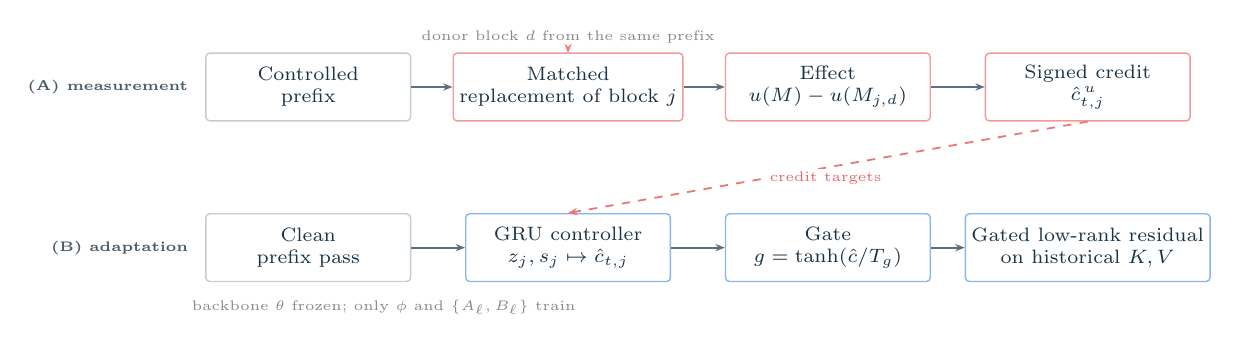
\begin{tikzpicture}[
  font=\scriptsize,
  x=1cm, y=1cm,
  box/.style={draw=linegray, line width=0.5pt, rounded corners=1.4pt,
              fill=pale, minimum height=0.86cm, minimum width=2.60cm,
              align=center, inner sep=2.2pt, text=ink},
  meas/.style={box, fill=white, draw=harmful!55},
  adap/.style={box, fill=white, draw=useful!55},
  srcline/.style={box, fill=white, draw=linegray},
  ar/.style={-{Stealth[length=3.4pt,width=2.6pt]}, line width=0.65pt,
             draw=ink!70},
  lab/.style={font=\tiny, text=muted, inner sep=1pt},
  lane/.style={font=\tiny\bfseries, text=ink2, inner sep=0pt},
]

% ---------------- lane A: measurement (supervision) ----------------
\node[lane, anchor=east] at (-1.52, 1.62) {(A) measurement};
\node[srcline] (A1) at (0.00, 1.62) {Controlled\\prefix};
\node[meas] (A2) at (3.30, 1.62) {Matched\\replacement of block $j$};
\node[meas] (A3) at (6.60, 1.62) {Effect\\$u(M)-u(M_{j,d})$};
\node[meas] (A4) at (9.90, 1.62) {Signed credit\\$\hat c^{\,u}_{t,j}$};

\draw[ar] (A1) -- (A2);
\draw[ar] (A2) -- (A3);
\draw[ar] (A3) -- (A4);

% the donor that feeds the replacement
\node[lab, anchor=south] at (3.30, 2.14) {donor block $d$ from the same prefix};
\draw[ar, draw=harmful!70] (3.30, 2.09) -- (3.30, 2.05);

% ---------------- lane B: adaptation (deployment) ----------------
\node[lane, anchor=east] at (-1.52, -0.42) {(B) adaptation};
\node[srcline] (B1) at (0.00, -0.42) {Clean\\prefix pass};
\node[adap] (B2) at (3.30, -0.42) {GRU controller\\$z_j,s_j\mapsto\hat c_{t,j}$};
\node[adap] (B3) at (6.60, -0.42) {Gate\\$g=\tanh(\hat c/T_g)$};
\node[adap] (B4) at (9.90, -0.42) {Gated low-rank residual\\on historical $K,V$};

\draw[ar] (B1) -- (B2);
\draw[ar] (B2) -- (B3);
\draw[ar] (B3) -- (B4);

% supervision flows from the measurement lane into the controller
\draw[ar, draw=harmful!75, dashed] (A4.south) --
  node[lab, right, pos=0.62, text=harmful!85, fill=white, inner sep=1.2pt]
  {credit targets} (B2.north);

% the frozen backbone applies to both lanes. The note sits below the lane-B
% boxes (whose bottom edge is y=-0.85) rather than under an arrowhead, which
% would have landed inside the last box.
\node[lab, anchor=north west] at (-1.52, -1.04)
  {backbone $\theta$ frozen; only $\phi$ and $\{A_\ell,B_\ell\}$ train};

\end{tikzpicture}%
}
\caption{\textbf{The \method\ pipeline.} Lane (A) is the measurement: a frozen
model scores a controlled prefix, one historical block's key span is replaced by
a matched donor, and the utility difference averaged over donors becomes the
credit target of Eq.~\eqref{eq:credit}. Lane (B) is the adaptation that consumes
it: a controller reads clean prefix features, predicts credit for every
historical block, and turns the prediction into a gate on a low-rank residual
applied to historical keys and values of Eq.~\eqref{eq:adapt}. The two lanes
share the intervention operator but not the tensors---the controller never sees
donor, effect or target-action information---and the weights of the frozen
backbone are never updated.}
\label{fig:pipeline}
\end{figure}




\section{Why the Objective Cannot Substitute for the Measurement}
\label{sec:divergence}

If action-score objectives already encoded memory usefulness, Eq.~\eqref{eq:credit}
would be an expensive way to recover something training gets for free. We test
that directly, using a precursor of our own method as the subject.

\begin{figure}[tbp]
\centering
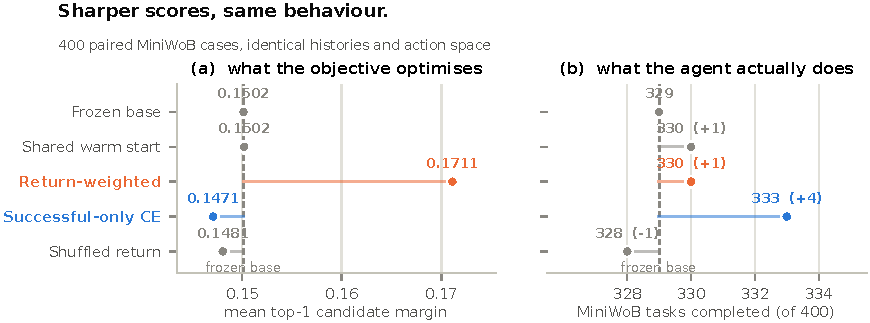
\includegraphics[width=\linewidth]{figures/fig4_divergence.pdf}
\caption{\textbf{The optimised score and the executed behaviour come apart.}
Four hundred paired MiniWoB cases, seeds 701--800, four task families, identical
histories and action space across arms. (a) The mean top-1 candidate margin.
(b) Tasks completed. Return-weighted training produces the largest margin and
does not convert it into completions; successful-only cross-entropy produces the
smallest margin and the most completions. Panels are dot plots because both
quantities have non-zero baselines.}
\label{fig:divergence}
\end{figure}

\paragraph{Setup.} \method's precursor applies return-conditioned KV adaptation
to a shared warm start on 41 training trajectories across three AndroidWorld
tasks, then trains five variants on identical data: return-weighted,
successful-only action cross-entropy, a shared warm start with no further
training, and a shuffled-return control. All arms are evaluated on the same 400
paired MiniWoB cases \citep{rawles2024androidworld}.

\paragraph{Result.} Return-weighted training moves the candidate margin from
$0.1502$ to $0.1711$, the largest of any arm, and ahead of a sign-flipped
control at $0.1481$ and successful-only CE at $0.1471$. It completes 330 of 400
tasks, against 329 for the frozen base and 333 for successful-only CE. Every
discrete difference in the entire comparison falls on the click-color family
(42, 43, 43, 46, 41 of 100 across arms); the other three families are saturated
or unchanged. The paired comparison against cross-entropy is $0$ rescues and $3$
regressions, an exact McNemar $p=0.25$ with a family-cluster interval of
$[-2.25, 0]$ percentage points, and all intervals include zero.

\paragraph{The same decoupling in the precursor itself.} The return-conditioned
KV arm lifts a held-out return margin from $0.1965$ to $0.2598$ over the shared
warm start, with sign-flipped labels at $0.1955$ and successful-only CE at
$0.1874$---the direction of the label clearly moves the metric. Top-1 action
ranking over those trajectories is $0.50$ for the frozen base, the
return-conditioned arm, the shuffled control and the cross-entropy arm alike.
The metric improved; the ranking did not.

\paragraph{Interpretation.} We do not conclude that return information is
useless for GUI memory. The precursor trains on 41 trajectories with 20
successes, its margin is measured on six held-out trajectories, and Appendix~\ref{app:precursor}
shows that random labels also improve the same offline score while a first-only
history is strongest---so the precursor's own diagnostic is not trustworthy at
this scale. What the two experiments establish is narrower and sufficient for
our argument: an objective can sharpen the quantity it optimises while leaving
behaviour at or below an untuned baseline, on paired data and within a single
seed. Whatever the score is measuring, it is not the agent's use of its history.
That gap is what Eq.~\eqref{eq:credit} is designed to close.

\section{Related Work}
\label{sec:related}

\paragraph{GUI memory and long-horizon interaction.} Agent Workflow Memory learns
reusable action routines and exposes selected workflows to later tasks
\citep{wang2024awm}. Latent approaches move the interface from text to continuous
representations: FocusMem separates content formation, state-conditioned readout
and evidence trust under a frozen GUI policy \citep{zhang2026focusmem}, and its
trust module explicitly addresses misleading retrieved evidence. We therefore do
not claim that selective memory or gating is new. The distinguishing element here
is the supervision signal: a measured signed effect of replacing an existing
historical decoder span at a fixed decision prefix, rather than a relevance or
trust label attached to an external memory item.

\paragraph{Internal interventions and representation adaptation.} Activation
patching measures the consequence of controlled internal substitutions, with
conclusions sensitive to the corruption and the metric
\citep{zhang2024patching}. ReFT learns task-specific representation
interventions while base weights stay frozen \citep{wu2024reft}, and visual
work shows how an internal representation pathology can motivate an
architectural remedy \citep{darcet2024registers}. \method\ adopts the same
observation-then-remedy separation; low rank limits the parameter and
perturbation budget but is not the source of the causal signal.

\paragraph{Capability-selective self-distillation.} SPD derives a capability
subspace from correctness gradients, steers KV during self-generation, and
finetunes on the resulting sequences \citep{hao2026spd}. Our target is not a
shared generation subspace but the signed contribution of one historical span
under the current GUI prefix.

\paragraph{Memory-focused evaluation.} MemGUI-Bench varies task conditions to
test short- and long-term memory use \citep{liu2026memgui}; the Android-in-the-Wild
interaction data underlies this line of device-control evaluation
\citep{rawles2023aitw}, and AndroidWorld evaluates state-changing mobile actions
\citep{rawles2024androidworld}; WorkArena++ stresses compositional workflows
\citep{boisvert2024workarena}.
These settings motivate measuring task outcomes rather than treating accuracy on
a synthetic recognition task as an application result---which is why our own
end-task evidence is reported as a boundary rather than a headline.

\section{Discussion}
\label{sec:discussion}

\paragraph{What a negative credit means.} It means a specified replacement
improves a specified utility under the tested prefix. The superseded record may
remain useful for a different question, and a small effect may reflect
redundancy rather than irrelevance. Whole-block effects do not decompose
additively: removing one supporting block can change another's contribution.
\method\ predicts credit from the complete observed history for this reason, and
its sign is tested under donor and template shifts rather than assumed stable.

\paragraph{Measurement scope.} Equal-length patching preserves the sequence
interface, not the full activation distribution. Donors carry context from
elsewhere in the prefix, and effects propagate through later layers. The reported
diagnostics are within-forward donors for the pilot and clean-prefill donors for
training, recorded separately. Two controls that would tighten the estimand have
not been run: a token-position control, and multi-donor sensitivity on held-out
templates. We therefore treat the sign and magnitude as established for the
donor distributions actually used, and not yet as invariant to them.

\paragraph{Boundary on the method.} \method's end-task benefit is not
established. On a sealed controlled test of the same family used here, the
adapted arm scores 23/200 against 24/200 for its matched control at equal
capacity, with a marginally better mean action NLL ($0.412004$ vs $0.412617$);
on the native mobile benchmarks, completed episodes stand at 0/21 for the
adapted arm against 1/21 for cross-entropy, on a base policy whose failures are
dominated by interface and infrastructure faults rather than memory handling.
We report \method\ as a framework that operationalises a validated measurement,
not as a benchmark win, and Appendix~\ref{app:native} gives the full protocol,
failure attribution and infrastructure record. The gap between identifying an
interfering memory and profitably rewriting it is the central open problem this
paper leaves.

\section{Conclusion}
\label{sec:conclusion}

GUI memory is not adequately described by what a model retains. In controlled
histories, the internal representation of a superseded update interferes with
the current decision while the correction sits in the same context window, and
the sign of a block's contribution is set by its relation to the decision rather
than by how old it is. That contribution is measurable per instance, is
invisible to the objectives currently used to train GUI memory, and is
discriminative enough to localise which block to distrust. \method\ turns it into
supervision. The question it leaves open is the one worth asking next: once a
memory is identified as interfering, what correction actually helps?

\label{main-text-end}

\clearpage
\section*{AI use statement}
(This section is required and does not count toward the page limit.)

In this work, we used generative AI tools for the following tasks with required
disclosure: developing the conceptual framework and the causal estimand
presented in Section~\ref{sec:method}; formulating the mathematical claims and
their notation; proposing and refining the hypotheses tested in
Sections~\ref{sec:credit} and~\ref{sec:divergence}; and providing feedback on
the design of the analysis methodology. We have not used generative AI tools to
generate synthetic datasets, to provide critical ingredients for proving
mathematical claims, or to assist in the writing of proofs, and those tasks are
not applicable to this work, which contains no formal proofs. Additionally, we
used generative AI tools for the following tasks with recommended disclosure:
creating and modifying the scientific figures; creating and editing the plotting
and evidence-extraction code; drafting and revising parts of the manuscript
text; and summarising and analysing existing literature for the related-work
discussion. We have reviewed all AI-assisted work. All figures are regenerated
from source data by a single extraction script that treats a missing source file
as a hard error rather than substituting a default, every empirical quantity in
the main text is traced to a named experiment record in
Appendix~\ref{app:evidence}, and the generated plotting code was executed and its
output inspected at final reproduction size. Bibliography entries were carried
from the project's verified citation ledger rather than produced by a language
model; one internal inconsistency, a preprint identifier that disagreed with its
own URL, was found and corrected against that ledger. We take responsibility for
the final content of this work, including text, claims or artifacts produced
with the aid of generative AI.
% AUTHOR ACTION: confirm the review sentence above against the authors' own
% verification (the template suggests e.g. "code was verified and tested by 2
% authors") and complete the matching fields in the submission form.

\section*{Ethics Statement}
GUI agents can expose private information or perform consequential actions.
Evaluation should use sandboxed benchmark accounts and controlled environments,
not users' production applications. Stored screenshots and trajectories should be
minimised, access-controlled and redacted before release. Memory-credit
estimation and controller training must not give the agent privileged evaluator
state. Deployment beyond benchmarks requires authorisation boundaries and
independent checks for irreversible actions.

\section*{Reproducibility Statement}
Appendix~\ref{app:protocol} specifies splits, controller inputs, loss
definitions and matched evaluation conditions. Appendix~\ref{app:evidence} maps
every measured number in the main text to its experiment record. Figures
\ref{fig:intervention}, \ref{fig:credit}, \ref{fig:joint} and
\ref{fig:divergence} are generated by code in \texttt{plotting/}, which reads
the repository JSON records through a single extraction script and prints a
verification report; the figure inputs and the table values therefore share one
path. The method diagram (Figure~\ref{fig:pipeline}) is inline vector art in the
source. An anonymised snapshot of all of the above accompanies the submission
(Appendix~\ref{app:completion}).

\begin{thebibliography}{99}
\bibitem[Bai et~al.(2025)]{bai2025qwen}
Shuai Bai, Keqin Chen, Xuejing Liu, Jialin Wang, Wenbin Ge, Sibo Song, et~al.
Qwen2.5-VL technical report. \emph{arXiv preprint arXiv:2502.13923}, 2025.
\url{https://arxiv.org/abs/2502.13923}.

\bibitem[Boisvert et~al.(2024)]{boisvert2024workarena}
L\'eo Boisvert, Megh Thakkar, Maxime Gasse, Massimo Caccia, Thibault Le Sellier De Chezelles, Quentin Cappart, Nicolas Chapados, Alexandre Lacoste, and Alexandre Drouin.
WorkArena++: Towards compositional planning and reasoning-based common knowledge work tasks.
\emph{arXiv preprint arXiv:2407.05291}, 2024.
\url{https://arxiv.org/abs/2407.05291}.

\bibitem[Darcet et~al.(2024)]{darcet2024registers}
Timoth\'ee Darcet, Maxime Oquab, Julien Mairal, and Piotr Bojanowski.
Vision transformers need registers. In \emph{International Conference on Learning Representations}, 2024.
\url{https://arxiv.org/abs/2309.16588}.

\bibitem[Hao et~al.(2026)]{hao2026spd}
Guangya Hao, Yitong Shang, Yunbo Long, Zhuokai Zhao, and Hanxue Liang.
Self-policy distillation via capability-selective subspace projection.
\emph{arXiv preprint arXiv:2605.22675}, 2026.
\url{https://arxiv.org/abs/2605.22675}.

\bibitem[Hu et~al.(2021)]{hu2021lora}
Edward J. Hu, Yelong Shen, Phillip Wallis, Zeyuan Allen-Zhu, Yuanzhi Li, Shean Wang, Lu Wang, and Weizhu Chen.
LoRA: Low-rank adaptation of large language models.
\emph{arXiv preprint arXiv:2106.09685}, 2021.
\url{https://arxiv.org/abs/2106.09685}.

\bibitem[Liu et~al.(2026)]{liu2026memgui}
Guangyi Liu, Pengxiang Zhao, Yaozhen Liang, Qinyi Luo, Shunye Tang, Yuxiang Chai, Weifeng Lin, Han Xiao, WenHao Wang, Siheng Chen, Zhengxi Lu, Gao Wu, Hao Wang, Liang Liu, and Yong Liu.
MemGUI-Bench: Benchmarking memory of mobile GUI agents in dynamic environments.
\emph{arXiv preprint arXiv:2602.06075}, 2026.
\url{https://arxiv.org/abs/2602.06075}.

\bibitem[Rawles et~al.(2023)]{rawles2023aitw}
Christopher Rawles, Alice Li, Daniel Rodriguez, Oriana Riva, and Timothy Lillicrap.
Android in the wild: A large-scale dataset for Android device control.
\emph{arXiv preprint arXiv:2307.10088}, 2023.
\url{https://arxiv.org/abs/2307.10088}.

\bibitem[Rawles et~al.(2024)]{rawles2024androidworld}
Christopher Rawles, Sarah Clinckemaillie, Yifan Chang, Jonathan Waltz, Gabrielle Lau, Marybeth Fair, Alice Li, William Bishop, Wei Li, Folawiyo Campbell-Ajala, Daniel Toyama, Robert Berry, Divya Tyamagundlu, Timothy Lillicrap, and Oriana Riva.
AndroidWorld: A dynamic benchmarking environment for autonomous agents.
\emph{arXiv preprint arXiv:2405.14573}, 2024.
\url{https://arxiv.org/abs/2405.14573}.

\bibitem[Wang et~al.(2024)]{wang2024awm}
Zora Zhiruo Wang, Jiayuan Mao, Daniel Fried, and Graham Neubig.
Agent workflow memory. \emph{arXiv preprint arXiv:2409.07429}, 2024.
\url{https://arxiv.org/abs/2409.07429}.

\bibitem[Wu et~al.(2024)]{wu2024reft}
Zhengxuan Wu, Aryaman Arora, Zheng Wang, Atticus Geiger, Dan Jurafsky, Christopher D. Manning, and Christopher Potts.
ReFT: Representation finetuning for language models.
\emph{arXiv preprint arXiv:2404.03592}, 2024.
\url{https://arxiv.org/abs/2404.03592}.

\bibitem[Zhang and Nanda(2024)]{zhang2024patching}
Fred Zhang and Neel Nanda.
Towards best practices of activation patching in language models: Metrics and methods.
In \emph{International Conference on Learning Representations}, 2024.
\url{https://arxiv.org/abs/2309.16042}.

\bibitem[Zhang et~al.(2026)]{zhang2026focusmem}
Zhuoran Zhang, Bowen Li, Jingcheng Ju, Yang Shi, Qixun Wang, Haotian Wang, Wei Chen, and Tengjiao Wang.
FocusMem: Factorizing content, readout, and trust in latent GUI memory.
\emph{arXiv preprint arXiv:2608.04530}, 2026.
\url{https://arxiv.org/abs/2608.04530}.
\end{thebibliography}

\clearpage
\appendix
\section{Training, Intervention, and Evaluation Details}
\label{app:protocol}
\subsection{A reproducible default, not a retrospective optimum}
The schedule in Table~\ref{tab:protocol} is the fixed starting protocol for the
\method\ comparison. It is not the configuration that produced the signed-effect
measurements of \S\ref{sec:credit}, which used frozen Qwen2.5-VL-3B,
middle-layer K interventions, and the historical extractor identified in
Appendix~\ref{app:evidence}.

\begin{table}[h]
\caption{Default protocol and bounded validation search for the learned \method\
model. No setting here implies a completed run. $\lambda_E$ applies to the
normalised energy of Eq.~\eqref{eq:energy} and cannot be copied numerically from
a differently normalised loss.}
\label{tab:protocol}
\centering\small
\begin{tabular}{L{.33\linewidth}L{.57\linewidth}}
\toprule
Item & Specification\\
\midrule
Primary backbone & Qwen2.5-VL-3B-Instruct; revision pinned in run manifest\\
Scale replication & Qwen2.5-VL-7B-Instruct, same preprocessing and protocol\\
History budget & 5 past screenshots + current; 8/12-history sweeps\\
Historical / current pixel caps & 100{,}352 / 401{,}408; identical across matched arms\\
Controller & 256-dimensional projection and state, one GRU layer, two-layer credit head\\
Controller alternatives & Independent MLP and two-layer Transformer, parameter counts reported\\
Default intervention & Decoder K, zero-based layers 12--23\\
Residual & Rank 8, $\alpha=8$ in $\alpha/r$ scaling; zero-initialized output factor\\
Controller / joint epochs & 5 / 5; best checkpoint selected on validation task success\\
Optimizer & AdamW; LR $3\times10^{-4}$ (controller), $10^{-4}$ (residual), weight decay .01\\
Batching & 1 prefix, accumulation 8; single model process per GPU\\
Training seeds & 11, 23, 37\\
Evaluation seeds & 101, 202, 303; reset environment and episode memory each time\\
Rank / layer sweep & $r\in\{4,8,16\}$; early/middle/late thirds\\
Credit weights & $\lambda_c=1$, $\lambda_s=.2$, $\lambda_r=.1$ initially; bounded validation sweep\\
Energy weight & $\lambda_E\in\{0,10,100,1000,3000\}$ for the stated normalization\\
Gate temperature & $T_g\in\{.5,1,2\}$ after training-only target scaling\\
Stage selection & No test-based temperature, donor, layer, or epoch selection\\
\bottomrule
\end{tabular}
\end{table}

\subsection{Prefix-only feature contract}
For every training prefix, record an immutable identifier, task group, screenshot
hashes, image order, prior actions, model revision, prompt, tokenized prefix
length, and visual-token spans. Feature extraction stops before target-action
tokens. Regression labels, success flags, candidate Q-values, semantic memory
roles, and evaluator metadata are not appended to the controller context. All
candidate actions at one prefix reuse identical features, and permuting candidate
order must not change those features or the predicted credit vector.

\subsection{Donor controls and uncertainty}
Match donors by projection dimension and token-span length; preserve recipient
positions and document any interpolation. The principal extractor does not
interpolate unequal spans. Use at least two distinct admissible donors where
available. Self-patching is an identity control. Same-forward donors and
clean-prefill donors are different protocols and have separate output records.

For donor effects $e_{t,j,d}=u(M_t)-u(\mathcal P_{j,d}(M_t))$, retain every
effect, the mean, sign agreement, absolute magnitude, donor identifiers and
sampling settings. Bootstrap over donors measures donor sensitivity, not
uncertainty over tasks; with two donors it is descriptive. The 200-prefix data
use two reference donors for non-reference blocks and one other reference donor
for a reference block, so reference-mean neutrality does not establish robust
instance-level neutrality---which is why \S\ref{sec:credit} reports per-instance
joint signs and absolute magnitudes alongside the means.

\subsection{Native rollout credit}
For a restorable training state, execute $K$ paired continuations per
intervention arm:
\begin{equation}
 \hat c^{\mathrm{roll}}_{t,j}=\frac{1}{DK}\sum_{d=1}^{D}\sum_{k=1}^{K}
 \big[R(\tau^{\mathrm{base},k})-R(\tau^{\mathrm{patch}(j,d),k})\big].
\end{equation}
Use matched environment state and random-number streams where feasible, fix
whether the patch applies only at the current decision or persists into later
decisions, and report restoration checks. Real-device retries are not independent
samples if state restoration failed. This estimator is specified but has not been
executed: every credit measurement in this paper uses the offline utilities of
Eqs.~\eqref{eq:act} and~\eqref{eq:val}, and no native rollout credit on
restorable states is reported. The performance-linked version of the estimand
therefore remains untested, and \S\ref{sec:discussion} treats that as a scope
limit rather than a result.

\section{Training and Deployment Procedure}
\label{app:algorithm}
Algorithm~\ref{alg:sigma} states the full procedure referenced by \S\ref{sec:sigma}: measurement of signed credit, controller fitting, joint optimisation of the gated residual, and the deployment loop. The selection rule in line~15 is the one the paper actually uses; no test-based donor, layer or epoch selection is performed.

\begin{algorithm}[H]
\caption{\method: learning memory adaptation from interventions}
\label{alg:sigma}
\small
\setlength{\tabcolsep}{0pt}
\renewcommand{\arraystretch}{1.16}
\begin{tabular}{@{}r@{\hspace{0.55em}}L{0.915\linewidth}@{}}
\textbf{1} & \textbf{Require:} training prefixes $\mathcal H$; frozen VLM $\theta$; donor pool $\mathcal D$; utility $u$\\
\textbf{2} & \textbf{Require:} controller $\phi$; residual factors $\{A_\ell,B_\ell\}_{\ell\in\mathcal L}$; weights $\lambda_c,\lambda_E$\\
\textbf{3} & \textbf{for} each $h_t\in\mathcal H$ \textbf{do}\\
\textbf{4} & \hspace{1.0em}Encode the clean prefix; record $M_t$, visual spans and decision features $q_t$\\
\textbf{5} & \hspace{1.0em}\textbf{for} historical block $j$ and admissible donor $d$ \textbf{do}\\
\textbf{6} & \hspace{2.0em}Evaluate $u(h_t;M_t)-u(h_t;\mathcal P_{j,d}(M_t))$ against the frozen copy of the prefix\\
\textbf{7} & \hspace{1.0em}\textbf{end for}\\
\textbf{8} & \hspace{1.0em}Aggregate effects and donor dispersion into credit targets $\tilde c^u_{t,j}$ and signs $y_{t,j}$\\
\textbf{9} & \textbf{end for}\\
\textbf{10} & Fit $\phi$ alone on $\mathcal L_{\mathrm{credit}}$ of Eq.~\eqref{eq:credit-loss}, with the residual held at identity ($A_\ell=0$)\\
\textbf{11} & \textbf{for} each joint epoch \textbf{do}\\
\textbf{12} & \hspace{1.0em}Sample prefixes; predict $g_{t,j}$ from clean features only; apply Eq.~\eqref{eq:adapt} to historical $K,V$\\
\textbf{13} & \hspace{1.0em}Update $\phi$ and $\{A_\ell,B_\ell\}$ on $\mathcal L_{\mathrm{SIGMA}}$ of Eq.~\eqref{eq:total}; $\theta$ stays frozen\\
\textbf{14} & \textbf{end for}\\
\textbf{15} & Select the checkpoint on validation tasks, never on evaluated tasks or donors\\
\textbf{16} & \textbf{Deploy:} predict gates once per step from a clean pass; generate; execute; reobserve and rebuild the prefix\\
\end{tabular}
\end{algorithm}

\section{Loss Definitions and Distillation}
\label{app:loss}
\paragraph{Within-prefix credit ranking.} For pairs whose teacher effects differ
by more than a calibrated tolerance, let $s_{ij}=\operatorname{sign}(\tilde c_i-\tilde c_j)$ and
\begin{equation}
 \mathcal L_{\mathrm{rank}}=
 \frac{1}{|\mathcal P|}\sum_{(i,j)\in\mathcal P}
 w_{ij}\log\big(1+\exp[-s_{ij}(\hat c_i-\hat c_j)]\big),\quad w_{ij}\ge0.
\end{equation}
A missing or uncertain label is masked, not silently treated as neutral.
Thresholds and target scales are fitted on the training/validation partition for
each utility type.

\paragraph{A finite replacement is not a scaling derivative.} If $f(x)=x-x^2$,
the original state $x=1/2$ has higher utility than the donor $x=0$, yet
$f'(1/2)=0$ and increasing $x$ reduces utility. A positive finite replacement
credit therefore does not justify an arbitrary positive displacement. In
attention, multiplying a key by $1+\eta$ changes a query logit by
$\eta q^\top k/\sqrt d$, whose sign depends on $q^\top k$. Equation~\eqref{eq:total}
optimises the action effect of the residual separately from the credit predictor
for this reason, and the paper nowhere identifies a signed gate with a proven
beneficial intervention.

\paragraph{No-hook policy distillation.} Let $p_T$ be the adapted teacher and
$p_S$ a same-architecture LoRA student \citep{hu2021lora}. Ordinary policy
distillation minimises
\begin{equation}
 \mathcal L_{\mathrm{KD}}=\E_h w_h\,\KL(\sg[p_T(\cdot\mid h)]\,\|\,p_S(\cdot\mid h)),\qquad w_h\ge0,
\end{equation}
with candidate-distribution and token-distribution KL reported as separate
interfaces. Residual distillation uses centered logits with
$P=I-\mathbf 1\mathbf 1^\top/C$ for $C$ candidates:
\begin{equation}
 \mathcal L_{\mathrm{res}}=\E_h w_h
 \big\|P(z_S-z_0)-\sg[P(z_T-z_0)]\big\|_2^2
 +\lambda_0\KL(p_0\|p_S).
\end{equation}
Centering removes arbitrary common logit shifts. Signed return baselines are not
used as negative coefficients on a KL loss. Static merging is a different
operation: a fixed residual $y'=(I+AB)y$ folds into $W'=(I+AB)W$, but a
history-dependent factor $g(h)$ cannot generally be represented by one constant
weight matrix, so the earlier merged-student result is not evidence that the
recurrent controller has been distilled away. The no-hook student itself has not
been trained: it is worth attempting only behind a measured teacher gain, which
\S\ref{sec:discussion} reports as not established, so we specify the objective
and leave it untested rather than claim a deployment saving.

\section{Evidence Ledger}
\label{app:evidence}
Table~\ref{tab:evidence} maps every measured number in the main text to its
record. The extraction script \texttt{plotting/extract\_evidence.py} reads these
files, writes the figure and table inputs, and prints a verification report; a
missing source file is a hard error rather than a defaulted value.

\begin{table}[h]
\caption{Evidence boundaries used throughout the manuscript. Record paths are
breakable so that no filename can run into the margin.}\label{tab:evidence}
\centering\footnotesize
\begin{tabular}{@{}L{.225\linewidth}L{.345\linewidth}L{.325\linewidth}@{}}
\toprule
Main-text object & Source record & Scope and limitation\\
\midrule
Fig.~\ref{fig:intervention}, Table~\ref{tab:pilot} &
\path{tango_v4_interference_chain_kv_credit_pilot10.json} &
10 paired prefixes, within-forward matched donors; pilot scale\\
Table~\ref{tab:credit}, Fig.~\ref{fig:credit}, Fig.~\ref{fig:joint} &
\path{tango_v2_teacher_credit200.json} &
200 prefixes, 1{,}000 blocks; candidate-value proxy, not native return\\
Fig.~\ref{fig:divergence} &
\path{tango_miniwob_click4_s701_800.json} &
400 paired cases; earlier global-return policy, not \method\\
\S\ref{sec:divergence} margin/ranking &
\path{gonogo_current.json} &
6 held-out trajectories; offline margin only\\
\S\ref{sec:discussion} boundary &
\path{docs/EXPERIMENT_STATUS_2026-09-17.md} &
Sealed controlled test, 3B\\
App.~\ref{app:native} native status &
\path{docs/SIGMA_BENCHMARK_EXPERIMENT_LOG_2026-09-18.md} &
Incomplete episodes; infrastructure faults present\\
\bottomrule
\end{tabular}
\end{table}

\section{Native GUI Evaluation Status}
\label{app:native}
This appendix records why the method's end-task claim is a boundary rather than
a result. It is included because the manuscript should not be read as asserting
an unmeasured gain.

\paragraph{Controlled sealed test.} On a sealed template-C test of 200 prefixes,
the adapted arm scores 23/200 against 24/200 for its matched control, with mean
action NLL $0.412004$ against $0.412617$. Validation had selected the same arm
at $0.18$ against $0.16$. This is a no-go for a discrete accuracy claim, and the
sealed test was not reused for further selection.

\paragraph{Native benchmarks.} The evaluated configuration is a frozen
Qwen2.5-VL-7B-Instruct backbone with 930{,}305 trainable parameters (controller
856{,}577; residual 73{,}728), decoder-K intervention at layers 9--17, rank 8,
$\alpha=8$, and a single 256-wide GRU layer. Training used 200 controlled
prefixes per arm with 50 validation prefixes; all six selected checkpoints reach
100\% candidate accuracy on those validation prefixes, which is a controlled
slot-selection number and not a task-success rate. At the time of the log,
completed episodes stood at 0/5 (new action protocol) and 0/19 (retired
protocol) for AndroidWorld, and 0/21 for the adapted arm against 1/21 for
cross-entropy on MemGUI under a registered alternate-judge protocol.

\paragraph{Failure attribution.} These failures are not cleanly attributable to
memory handling. In the AndroidWorld new-protocol episodes, all 150 executed
steps were \texttt{answer} actions with zero illegal actions---the base policy
never attempted a tap or text entry---so a first-step action error cannot be
ascribed to history selection, and the first step has no historical image at
all. Recorded infrastructure faults include an emulator clock regression of
$34.5$ hours after snapshot restore, a backend HTTP~500 on empty text input, and
judge rate limiting; repair patches for the clock and gesture issues were
verified but several landed mid-batch, so affected episodes use different
effective environment revisions. Denominators here count completed episodes, not
task types, and the batches are incomplete. We therefore report these numbers as
a status record, not as a method comparison.

\section{Precursor Results}
\label{app:precursor}
These experiments concern earlier global-return and action-credit variants and are
not mixed with \method. They document why the final evaluation uses task success
rather than confidence sharpening.

\begin{table}[h]
\caption{Observed MiniWoB success counts. Each family has 100 common seeds,
giving 400 paired task instances per method. All model differences occur in
click-color; the other three families are unchanged or saturated.}
\label{tab:miniwob}
\centering\small
\begin{tabular}{lrrrrr}
\toprule
Task family & Base & Warm & Global return & Success CE & Shuffle\\
\midrule
click-button &97&97&97&97&97\\
button-sequence &90&90&90&90&90\\
click-color &42&43&43&46&41\\
click-tab &100&100&100&100&100\\
\midrule
Total &329&330&330&333&328\\
Success (\%) &82.25&82.50&82.50&83.25&82.00\\
\bottomrule
\end{tabular}
\end{table}

Table~\ref{tab:miniwob} gives the per-family counts. Global return versus success
CE has zero rescues and three regressions, with
exact paired McNemar $p=.25$; versus the warm start it has two rescues and two
regressions. The family-cluster interval versus CE is $[-2.25,0]$ percentage
points based on four families and should not be read as a precise estimate for a
broad population of GUI tasks. Mean candidate margins are $.15017$ for Base,
$.17110$ for global return, and $.14712$ for CE.

\begin{table}[h]
\caption{Observed AndroidWorld offline controls on six held-out trajectories.
These are return-margin diagnostics, not task-success rates.}
\label{tab:android}
\centering\small
\begin{tabular}{lr@{\hspace{1cm}}lr}
\toprule
Target & Margin & Training range & Margin\\
\midrule
Warm start & .13015 & $H=1$ & .13975\\
Normal return & .14116 & $H=3$ & .14387\\
Shuffled return & .13219 & $H=5$ & .14304\\
Random return & .13745 & Full trajectory & .14309\\
Sign-flipped return & .12312 & First-only & .14663\\
 & & Final-only & .13843\\
 & & Remove history & .13786\\
\bottomrule
\end{tabular}
\end{table}

Table~\ref{tab:android} reports the returned-margin controls.
Normal and sign-flipped labels move the offline score in opposite directions, but
random labels also improve it and the first-only condition is strongest. These
measurements motivate the stricter comparison of \S\ref{sec:divergence}; they do
not identify the cause of the precursor's online outcome, and they do not prove
that a correctly implemented on-policy return estimator cannot localise useful
credit.

\paragraph{Transport and gate observations.} An energy-regularised variant of
the precursor reduces measured activation transport energy by $4.47\times$
($0.3004\times10^{-3}\to0.0672\times10^{-3}$) while retaining 97.8\% of the
unregularised return margin. Its learned gate magnitudes over history slots are
$0.418\to0.179\to0.078$ for the distractor-credit family and
$0.704\to0.039\to0.290$ for the hidden-memory family: the first decays
monotonically with distance from the current decision and the second does not.
With 20--240 prefixes per cell and a single training run, we treat this as a
descriptive observation about one trained controller, not as evidence for a
general recency rule, and it is not used to support any main-text claim.

\section{Figures and Data Availability}
\label{app:completion}
Figures~\ref{fig:intervention}, \ref{fig:credit}, \ref{fig:joint} and
\ref{fig:divergence} are produced by matplotlib code in \texttt{plotting/}, with
the shared visual system in \texttt{style.py}; the categorical and diverging
palettes used there pass a colour-vision-deficiency separation check and every
value is drawn from \texttt{data/}, which is generated by
\texttt{plotting/extract\_evidence.py}. The method diagram
(Figure~\ref{fig:pipeline}) is inline vector art in the source. No figure in this
paper is generated imagery, and no missing value is rendered as a plotted point.

The supplementary archive contains the manuscript source, the plotting and
extraction code, the extracted figure inputs, and the upstream experiment
records the extraction reads. Running \texttt{extract\_evidence.py} and then the
four figure scripts regenerates every reported number and every quantitative
figure from those records, and the extraction prints a verification report rather
than silently defaulting a missing source. The archive contains no
author-identifying information: paths are derived from \texttt{\_\_file\_\_}, and
the staged tree is scanned for identifying strings before the archive is written.

\end{document}
